\documentclass{article}
\usepackage{fancyhdr}
\usepackage{amsmath,amssymb}
\usepackage{geometry}
\usepackage{datetime}
\usepackage{enumerate}
\usepackage{graphicx}

%Insert page formatting here
%\hoffset = -.5in
\voffset = -0.375in
%\textwidth = 6in
\textheight = 9in
\headheight = 24pt

\pagestyle{fancy}

\rhead{Peter Olson\\Student ID: $441666$}
\lhead{Math 3200\\Homework 5}
\chead{\today}
\cfoot{}

%\addtolength{\headwidth}{\marginparsep}
%\addtolength{\headwidth}{\marginparwidth}

%\renewcommand{\labelitemi}{$\diamond$}
\renewcommand{\implies}{\rightarrow}
\newcommand{\widespace}{\qquad \qquad \;}
\newcommand{\tret}{\\ \hline}
\newcommand{\fh}{\tfrac{1}{2}}
\newcommand{\deriv}[2]{\frac{d #1}{d #2}}
\newcommand{\pderiv}[2]{\frac{\delta #1}{\delta #2}}
\newcommand{\vr}{\vec{r}}
\newcommand{\at}{\text{ at }}
\newcommand{\var}{\text{Var}}

\begin{document}
	\section*{Exercise 5.27}
	The resulting quantiles are very close to the Student-T distribution of $t_{4}$. $t_4$ has:
	
	
	25th Percentile: -0.7407
	
	50th Percentile: 0.0000
	
	90th Percentile: 1.533
	
	\section*{Console Output}
	\begin{verbatim}
	> show(quantile(T, c(.25, .5, .9)))
	25%         50%         90% 
	-0.75984380 -0.01844971  1.40915035 
	\end{verbatim}
	\section*{Plot}
	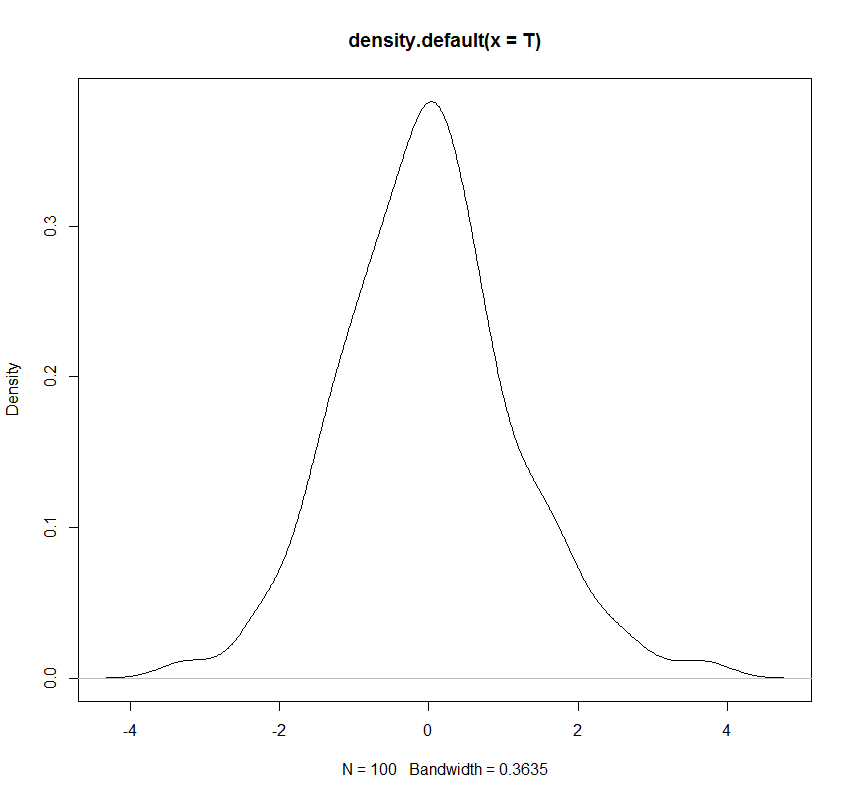
\includegraphics[width=4in]{q4}
	\section*{R Code}
	\begin{verbatim}
	mu    <- 10
	n     <- 5
	sigma <- 3
	
	dist_matrix <- matrix(nrow = 0, ncol = 5)
	
	for(i in 1:100){
	dist_matrix <- rbind(dist_matrix, rnorm(n, mu, sigma))
	}
	
	# mean_vector <- rowMeans(dist_matrix)
	mean_vector <- apply(dist_matrix, 1, mean)
	
	var_vector <- sqrt(apply(dist_matrix, 1, var))
	
	T <- (mean_vector - mu) * sqrt(n) / var_vector
	
	show(quantile(T, c(.25, .5, .9)))
	
	plot(density(T))
	\end{verbatim}
\end{document}